\begin{answer}
\begin{figure}[h!]
\centering
\begin{subfigure}{.5\textwidth}
  \centering
  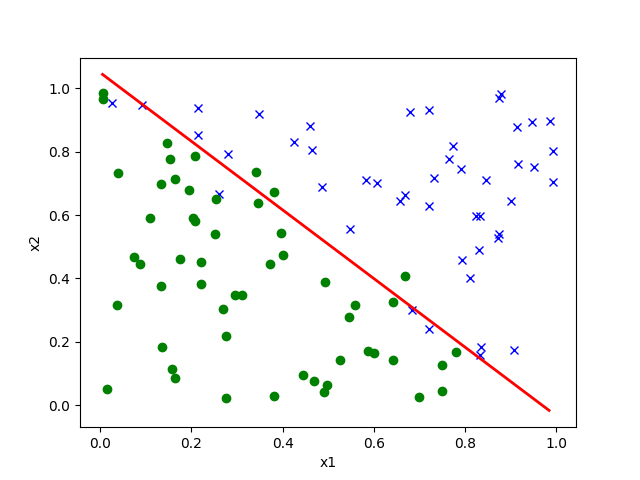
\includegraphics[width=.75\linewidth]{stability/0.png}
  \caption{Data A}
  \label{fig:sub1}
\end{subfigure}%
\begin{subfigure}{.5\textwidth}
  \centering
  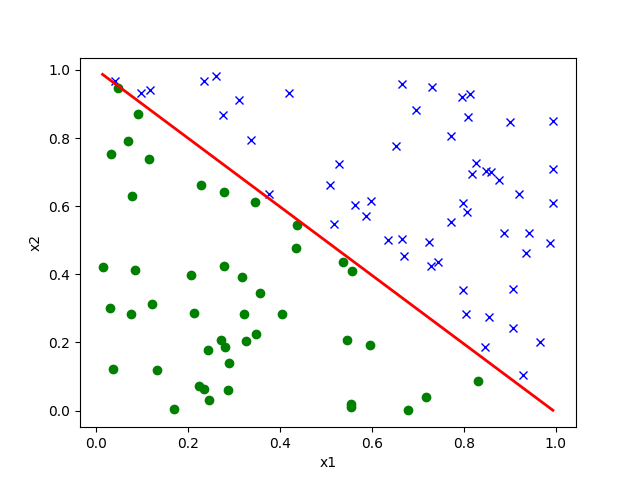
\includegraphics[width=.75\linewidth]{stability/1.png}
  \caption{Data B}
  \label{fig:sub2}
\end{subfigure}
\caption{Data B is perfectly seprable}
\label{fig:test}
\end{figure}

The reason is that dataset B is perfectly separable while A is not. LR without Regularisation as in the code will not converge to a single parameter because of the fact that it is perfectly separable. Since it is perfectly separable any $\theta$ \ that separates can decrease the loss but no change in boundary.
\\ \\

\end{answer}
